\documentclass[15pt]{beamer}
\usetheme{Warsaw}
\usepackage{enumitem}
\usepackage{multicol}
\usepackage{multirow}
\usepackage{graphics}
\usepackage[export]{adjustbox}
\usepackage{bookmark}



\setbeamercolor{normal text}{fg=white,bg=black!90}
\setbeamercolor{structure}{fg=white}

\setbeamercolor{alerted text}{fg=red!85!black}

\setbeamercolor{item projected}{use=item,fg=black,bg=item.fg!35}

\setbeamercolor*{palette primary}{use=structure,fg=structure.fg}
\setbeamercolor*{palette secondary}{use=structure,fg=structure.fg!95!black}
\setbeamercolor*{palette tertiary}{use=structure,fg=structure.fg!90!black}
\setbeamercolor*{palette quaternary}{use=structure,fg=structure.fg!95!black,bg=black!80}

\setbeamercolor*{framesubtitle}{fg=white}

\setbeamercolor*{block title}{parent=structure,bg=black!60}
\setbeamercolor*{block body}{fg=black,bg=black!10}
\setbeamercolor*{block title alerted}{parent=alerted text,bg=black!15}
\setbeamercolor*{block title example}{parent=example text,bg=black!15}




\title{Image Retrival by Comparing Color Features}


\author[Mamun \and Mahmudul]{Abdullah Al Mamun (1305003) \and \\ S. Mahmudul Hasan (1305043)}

\institute[BUET]{Bangladesh University of Engineering and Technology}

\date{\today}



\begin{document}
\section*{Greeting}
\subsection*{Title}



\begin{frame}
\titlepage
\end{frame}


\begin{frame}
\fontsize{18pt}{20}\selectfont
\centering
The original Research was done by:\\[\baselineskip]
S.R. Kodituwakku\footnote{University of Peradeniya}\\[\baselineskip]
\centerline{\&}\medskip
S.Selvarajah\footnote{University of Jaffna}
\end{frame}


\subsection*{Outline}
\begin{frame}
\frametitle{Outline}
%\begin{NoHyper}
\tableofcontents
%\end{NoHyper}
\end{frame}


\section{Problem}

\begin{frame}
\begin{center}
\Huge Problem
\end{center}
\end{frame}

\subsection{Image Retrieval}

\begin{frame}
\frametitle{What is Image Retrieval?}
\begin{itemize}[label=$\blacksquare$]
\item Retrieve image from database
\item Search by keywords or a query image\\[\baselineskip]
\pause
\item Our focus: Content Based Image Retrieval (CBIR)
\end{itemize}
\end{frame}

\begin{frame}
\frametitle{Content Based Image Retrieval}
\begin{itemize}[label=$\blacksquare$]
\item Search key is an \textbf{image}
\item Retrieve image comparing similarity
\end{itemize}
\end{frame}

\subsection{Application}
\begin{frame}
\frametitle{Application}
\begin{itemize}[label=$\blacksquare$]
\item Finding similar images
\item Retrieving a criminal's profile
\end{itemize}
\end{frame}

\begin{frame}
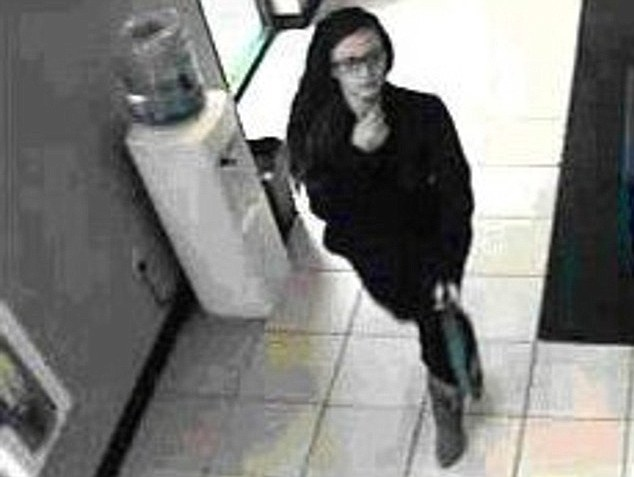
\includegraphics[scale=0.5,center]{criminal.jpg}
\end{frame}


\section{Proposal}
\begin{frame}
\begin{center}
\Huge Proposal
\end{center}
\end{frame}

\begin{frame}
\frametitle{Proposal}
Compare the Color Features
\end{frame}

\subsection{Color Features}
\begin{frame}
\frametitle{Color Features}
\pause
\begin{itemize}[label=$\blacksquare$]
\item Color Moments
\pause
\item Histogram
\pause
\item Color Coherent Vector (CCV)
\end{itemize}
\end{frame}


\begin{frame}

\frametitle{Color Moments}
\pause
\begin{itemize}[label=$\blacksquare$]
\item Mean
\pause
\item Variance
\pause
\item Standard Deviation
\pause
\end{itemize}

Let, \textit{$P_{ij}$} is the pixel value of the pixel on $i$th row and $j$th column.
\textit{N} is the number of pixels.\newline \newline
\pause
$mean = \frac{SUM(P_{ij})}{N}$
\end{frame}




\begin{frame}
\frametitle{Histogram}

\begin{itemize}[label=$\blacksquare$]
\item Tonal distribution of pixels.
\item Tonal range is a measurement of darkness or lightness \\[\baselineskip]\pause
\item Can be used to find the Color Moments
\item Used for very large datasets when direct methods are expensive
\end{itemize}
\end{frame}





\begin{frame}
\frametitle{Histogram}
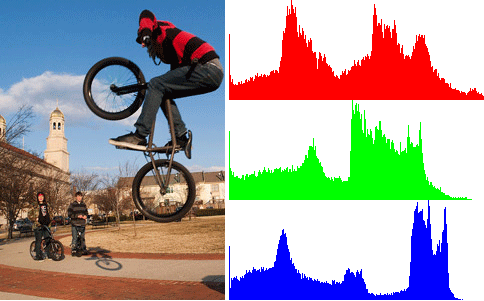
\includegraphics[scale=0.45,center]{jump_hist}
\newline\pause
Problems?
\begin{itemize}[label=$\blacksquare$]
\item Two different images may have almost same histogram.
\end{itemize}
\end{frame}


\begin{frame}
\frametitle{Color Coherent Vector (CCV)}
Differentiate every pixel into 2 categories:
\begin{itemize}[label=$\blacksquare$]
\item Coherent - neighborhood pixels have similar tonal range
\item Incoherent - otherwise \newline \newline
\end{itemize}
\pause
CCV represents this classification for each color.
\end{frame}

%------------2nd part starts here --------------------

\fontsize{9}{7}\selectfont


\section{Methodology}

\begin{frame}
\fontsize{18pt}{30}\selectfont
\centering
METHODOLOGY
\end{frame}

\subsection{Color Reduction}
\begin{frame}
\frametitle{Color Reduction}
\begin{itemize}[label=$\blacksquare$]
\pause
\item True Color: supports 24-bit for three RGB colors\\[\baselineskip]
\pause
\item Total number of possible colors: $2^{24}$\\[\baselineskip]
\pause
\item Reduced to: 256
\end{itemize}
\end{frame}

\subsection{Histogram Based Image Retrival}
\begin{frame}
\frametitle{Histogram Based Image Retrival}
Two techniques:\\[\baselineskip]
\pause
\begin{itemize}[label=$\blacksquare$]
\item GCH: Global Color Histogram
\pause
\item LCH: Local Color Histogram\\[\baselineskip]
\pause
\end{itemize}
GCH:\\[\baselineskip] Represents images with \textbf{single} histogram.\\[\baselineskip]
\pause
LCH:\\[\baselineskip] Images are divided into fixed blocks of \textbf{size 8x8} \& histogram is obtained for \textbf{each} block
\end{frame}



\begin{frame}
\frametitle{Histogram Based Image Retrival}
Steps for using histogram:\\
\pause
\begin{itemize}[label=$\blacksquare$]
\setlength\itemsep{1.2em}

\item Histograms of all images in the databes are computed \& stored
\pause
\item Histogram of the query image is computed
\pause
\item Measure similarity of database's images and query images using euclidian distance metrics
\pause
\item Identify relevant images using a fixed threshold value\\[\baselineskip]
\end{itemize}
\pause
\textbf{Euclidian Distance Metrics?}\\[\baselineskip]
\pause
For \textbf{3D}
\begin{equation}
distance((x,y,z),(a,b,c)) = \sqrt{(x-a)^2+(y-b)^2+(z-c)^2}
\end{equation}
\pause
Let,
Image A: $(x_1, x_2,\ldots,x_n)$\\
Image B: $(y_1, y_2,\ldots,y_n)$\\[\baselineskip]
\pause
Distance between A \& B = $\sqrt{\sum_{i=1}^{n}(x_i-y_i)^2}$
\end{frame}

\subsection{Extraction of Visual Feature}
\begin{frame}
\frametitle{Extraction of Visual Feature}
\pause
Extract viusal features using color histograms and moments \\[\baselineskip]
\pause
\begin{itemize}[label=$\blacksquare$]
\setlength\itemsep{1.5em}

\item Calculate mean and std. deviations of database images and store
\pause
\item Compare mean \& std. deviation of DB's images \& query image
\pause
\item Rank relevant images based on a fixed threshold value\footnote{Threshold value is based on the difference of the properties}\\[\baselineskip]
\end{itemize}
\end{frame}

\subsection{Coherence Bassed Image Retrival}
\begin{frame}
\frametitle{Coherence Measure}
Pixels: \textbf{Coherent} or \textbf{Incoherent}\\[\baselineskip]
\pause
Coherent pixels:\\
\pause
\begin{itemize}[label=$\blacksquare$]
\item Part of a sizable contiguous region
\pause

\item Compute \textbf{connected components} for pixel groups\footnote{A pixel and its 8 surrounding neighbours}

\pause
\item Size of a pixel group need to exceed a fixed value\footnote{1\% of the total image area} \\[\baselineskip]
\pause
\end{itemize}
Incoherent pixels: The rest of the pixels\\[\baselineskip]
Steps for image retrival:\\[\baselineskip]
\begin{itemize}[label=$\blacksquare$]
\pause
\item Classify pixels as coherent or incoherent.\\[\baselineskip]
\pause
\item Use a \textbf{color coherence vector} to represent those for each color.\\[\baselineskip]
\pause
\item Compute similarity between query \& DB's images CCVs and retrive.
\end{itemize}

\end{frame}

\begin{frame}
\fontsize{18pt}{30}\selectfont
\centering
RESULTS
\end{frame}


\section{Results}
\begin{frame}
\frametitle{Results}
\pause
General purpose image database containing 14500 images is used.\\[\baselineskip]
\pause
\textbf{Categories: }\\[\baselineskip]
\pause
\begin{multicols}{4}
    \begin{itemize}[label=$\blacksquare$]
        \item Africans \& villages
        \item Beaches
        \item Buildings
        \item Buses
        \item Dinosaurs
        \item Elephants
        \item Flowers
        \item Horses
        \item Mountains \& glaciers
        \item Foods
        \item Faces
        \item Objects
        \item Drawings
        \item Textures
        \item Natural scenes\\[\baselineskip]
    \end{itemize}
\end{multicols}
\pause
Image Details in the DB:
\pause
\begin{itemize}[label=$\blacksquare$]
\item Image Format:\textbf{ JPEG}\\
\pause
\item Imgae Size: \textbf{384x256}\\
\pause
\item Image Representation: \textbf{RGB color space}\\[\baselineskip]
\end{itemize}

\pause
\begin{description}[font=$\blacksquare$\scshape\bfseries]

\item[ Image used:] 5 per category 
\pause
\item[ Image Types :] Uniform, non-uniform \& average color distribution
\end{description}

\end{frame}




\begin{frame}
\frametitle{Results}
\pause
Performance Measurement Metrics:\\[\baselineskip]
\pause
\begin{itemize}[label=$\blacksquare$]
\item \textbf{Precision: }$\frac{Relevant\:retrived \:images}{Total \: retrived \: images}$
\pause
\item \textbf{Recall: }$\frac{Relevant \: retrived \: images}{Total \: relevant \: images  \:in \:DB}$
\end{itemize}
\fontsize{3}{5}\selectfont

\pause
\begin{table}
\caption{\textbf{Category - Dinosaurs}}

\resizebox{.6\columnwidth}{!}{
\begin{tabular}{|c|c|c|c|c|}
\hline
Descriptor & Recall & Precision\\
\hline
\multirow{2}{*}{\textbf{CM}} & 0.100137931 & 0.698748797\\
& 0.09862069 & 0.754219409\\
& 0.097586207 & 0.815092166\\
\hline
\multirow{2}{*}{\textbf{GCH}} & 0.099586207 & 0.529325513\\ & 0.09862069 & 0.580121704\\ & 0.096551724 & 0.615114236\\
\hline
\multirow{2}{*}{\textbf{LCH}} & 0.097586207 & 0.5\\ & 0.095586207 & 0.508064516\\
& 0.093586207 & 0.534672971\\
\hline
\multirow{2}{*}{\textbf{CCV}} & 0.10062069 & 0.555597867\\ & 0.099586207 & 0.585801217\\ & 0.096551724 & 0.631483987\\
\hline
\end{tabular}
}
\end{table}
\end{frame}


\begin{frame}
\fontsize{3}{5}\selectfont

\begin{table}
\caption{\textbf{Category - Africans}}

\resizebox{.8\columnwidth}{!}{
\begin{tabular}{|c|c|c|c|c|}
\hline
Descriptor & Recall & Precision\\
\hline
\multirow{2}{*}{\textbf{GCH \& CCV}} & 0.088531187 & 0.871287129\\
& 0.08249497 & 0.872340426\\
& 0.079476861 & 0.877777778\\
\hline
\multirow{2}{*}{\textbf{LCH \& CCV}} & 0.100603622 & 0.487804878\\
& 0.099597586 & 0.5\\
& 0.097585513 & 0.510526316\\
\hline
\multirow{2}{*}{\textbf{CCV, CM, LCH \& GCH}} & 0.095573441 & 0.95959596\\
& 0.09054326 & 0.97826087\\
& 0.088531187 & 0.988764045\\
\hline
\multirow{2}{*}{\textbf{GCH, LCH \& CCV}} & 0.098591549 & 0.439461883\\
& 0.096579477 & 0.507936508\\
& 0.095573441 & 0.50802139\\
\hline
\end{tabular}
}
\end{table}
\end{frame}



\begin{frame}
\fontsize{18pt}{30}\selectfont
\centering
DECISIONS
\end{frame}


\section{Decisions}
\begin{frame}
\frametitle{Decisions}
Which feature gives better performance?
\pause
\begin{description}[font=$\blacksquare$\scshape\bfseries]
\item[ Uniform Color Distribution: ] Color Histogram 
\pause
\item[ Average Color Distribution: ] Color Moments
\pause
\item[ Widely Scattered Colors: ] Color Coherent Vector\\[\baselineskip]
\end{description}
\pause
No feature is superior to other as performance is color distribution dependent.\\[\baselineskip]
\pause
\centerline{\textbf{But}}\medskip 
\pause
The \textbf{combination} of different descriptors gives most satisfactory results.
\end{frame}

\begin{frame}
\fontsize{18pt}{30}\selectfont
\centering
\textbf{Thank you!}\\[\baselineskip]
\textbf{Questions?}
\end{frame}





%\end{NoHyper}
\end{document}